\documentclass[a0]{4by3}
\usepackage{braket}
\usepackage{multicol,graphicx,color}
\usepackage{amsmath,amssymb,amsthm}
\usepackage{tabularx}
\usepackage{mathrsfs}
\usepackage{mathtools}
\usepackage{caption}
\usepackage{xparse}
\usepackage{enumerate}
\usepackage{tikz}
\usepackage{amsmath, amssymb, amsthm, amsfonts, algpseudocode, algorithm, bm, bbm, color, fixmath, float, graphicx, hyperref, listings, mathrsfs, mathtools, subfig} 
\usetikzlibrary{arrows.meta}
\newtheorem{theorem}{Theorem}
\newtheorem{definition}{Definition}
\newtheorem{corollary}{Corollary}
\newtheorem{problem}{Problem}
\newtheorem{conjecture}{Conjecture}
\newtheorem{approach}{Approach}
\newtheorem{lemma}{Lemma}
\newtheorem{idea}{Idea}
\newtheorem*{prop}{Result}
\newtheorem*{cor}{Corollary}
\newcommand{\defeq}{\vcentcolon=}
\usepackage{amsmath, amssymb, amsthm, amsfonts, algpseudocode, algorithm, bbm, color, fixmath, float, graphicx, hyperref, listings, mathrsfs, mathtools, subfig} 

%Needed commands
\newcommand*{\w}{\mathbf{w}}
\newcommand*{\x}{\mathbf{x}}
\newcommand*{\y}{\mathbf{y}}
\newcommand*{\z}{\mathbf{z}}
\newcommand*{\R}{\mathbb{R}}
\newcommand*{\E}{\mathbb{E}}
\newcommand*{\0}{\mathbf{0}}
\newcommand*{\minimizer}{\mathbf{x}^*}
\newcommand*{\dprime}{{\prime\prime}}
\newcommand{\li}[1]{\lstinline[prebreak=]!#1!}
\newcommand{\pseudoli}[1]{\lstinline[style=pseudo]!#1!}
\newcommand{\trp}{^{\mathsf T}} 
\newcommand{\im}{{i\mkern1mu}}
\newcommand{\Real}{\mathchardef\Re="023C}
\newcommand{\Imag}{\mathchardef\Im="023D}
\newcommand\norm[1]{\left\lVert#1\right\rVert}
\newcommand*\diff{\mathop{}\!\mathrm{d}}
\newcommand*\Eval[3]{\left.#1\right\rvert_{#2}^{#3}}

%Operators
\DeclareMathOperator{\argmin}{argmin}
\DeclareMathOperator{\argmax}{argmax}

%Link set up
\hypersetup{
    colorlinks=true, %set true if you want colored links
    linktoc=all,     %set to all if you want both sections and subsections linked
    linkcolor=blue,  %choose some color if you want links to stand out
    pdftitle={RL Notes},
    pdfpagemode=FullScreen
}

\endinput

%%%%%%%%%%%%%%%%%%%%%%%%%%%%%%%%%%%%
% VARIABLES & LAYOUT CONFIGURATION %
%%%%%%%%%%%%%%%%%%%%%%%%%%%%%%%%%%%%

% Colors
%%%% THIS IS WHERE YOU CAN CHANGE COLORS. 
\definecolor{titlebackground}{rgb}{0.0, 0.0, 0.5}
\definecolor{titletext}{rgb}{1, 1, 1}
\definecolor{titlesubtext}{rgb}{0.52, 0.586, 0.664}
\definecolor{subtitleoutline}{rgb}{0.0, 0.0, 0.5}
\definecolor{subtitlebackground}{rgb}{0.86, 0.84, 0.82}
\definecolor{subtitletext}{rgb}{0.0, 0.0, 0.5}
% Colors

% Columns
%%%% THIS IS WHERE YOU CAN CHANGE THE HEIGHT & NUMBER OF COLUMNS
\newcommand{\ColumnScale}{0.74526}
\newcommand{\NumColumns}{4}
\setlength{\fboxsep}{1cm}
\setlength{\columnsep}{3cm}
\color{titlesubtext}
\setlength{\columnseprule}{2mm}
\setlength{\fboxsep}{1cm}
\setlength{\fboxrule}{5mm}
% Columns

% Font Helvetica
\renewcommand\sfdefault{phv}
\renewcommand\familydefault{\sfdefault}
% Font Helvetica

% Math
\setlength{\abovedisplayskip}{5pt}
\setlength{\belowdisplayskip}{5pt}
% Math

%%%%%%%%%%%%%%%%%%%%%%%%%%%%%%%%%%%%
% FANCY COMMANDS                   %
%%%%%%%%%%%%%%%%%%%%%%%%%%%%%%%%%%%%

% Create the fancy title command
\NewDocumentCommand{\FancyTitle}{ O{1.25cm} m m m }{
    \noindent
    \colorbox{titlebackground}{\begin{minipage}{\dimexpr\textwidth+\fboxsep+2\fboxrule\relax-2\fboxsep}
      \begin{center}\vspace{5mm}
       {\VeryHuge \textcolor{titletext}{#2}}\\[10mm]
       {\Huge \textcolor{titletext} {#3}}\\[10mm]
       {\Large \textcolor{titletext}{#4}}
      \end{center}
    \end{minipage}}
    \vspace{#1}
}

% Create the fancy subtitle command
\NewDocumentCommand{\FancySubtitle}{ O{1cm} O{1cm} m }{
    \vspace{#2}
    \noindent
    \fcolorbox{subtitleoutline}{subtitlebackground}{\begin{minipage}{\dimexpr\linewidth-2\fboxsep-2\fboxrule\relax}
        \centering
        \sf \huge \textcolor{subtitletext}{#3}
    \end{minipage}}
    \vspace{#1}
}

% Create the fancy figure command
\NewDocumentCommand{\FancyFigure}{ O{0.9} m m m }{
    \begin{center}
        \begin{minipage}{#1\linewidth}
          \centering
          \includegraphics[width=\linewidth]{#2}
          \captionof{figure}{#3}
          \label{#4}
        \end{minipage}
    \end{center}
}

%%%%%%%%%%%%%%%%%%%%%%%%%%%%%%%%%%%%

\begin{document}

\FancyTitle{Smart Dosing}{Optimal Control of AC Treatment in IDC}{Óscar J. Escobar, Joseph Humpherys, Henry Fetzer, Clifton Langley}
%Main
\color{black}
\noindent
\begin{minipage}{\linewidth + 2\fboxsep}
\begin{multicols*}{\NumColumns}
    \FancySubtitle[5mm]{Overview}
        \large
        
        \indent Mathematical Oncology (MO) is described as a ``a bridge between $\ldots$ the biologist and practician clinician " [RR19].
        Tumor modeling is an area of MO whose objective is to create and understand models that can help clinicians understand properties that govern tumor growth, the effects of treatments, and other factors like toxicity to the person, or the affects of the immune system on cancerous tumor. 
        However, the majority of models do not look into personalized treatments that can be adaptive to the response of a person as the modeling focuses in understanding dynamics.\\
        
        \indent Optimal control theory (OTC) seeks to find the best possible control strategy for a dynamical system by optimizing a performance criterion while following constraints and dynamics of system.
        OTC can be combined with tumor modeling by leaving the chemotherapy unknown so that solving the optimizing problem according to tumor modeling constraints can help us find a personalized chemotherapy function.
        This would help us examine better how certain treatments affect the tumor and the patient as we vary the chemotherapy administered. 
    \vspace{-17mm}
    
    \FancySubtitle[0cm][2cm]{The problem}
            \large 
            
             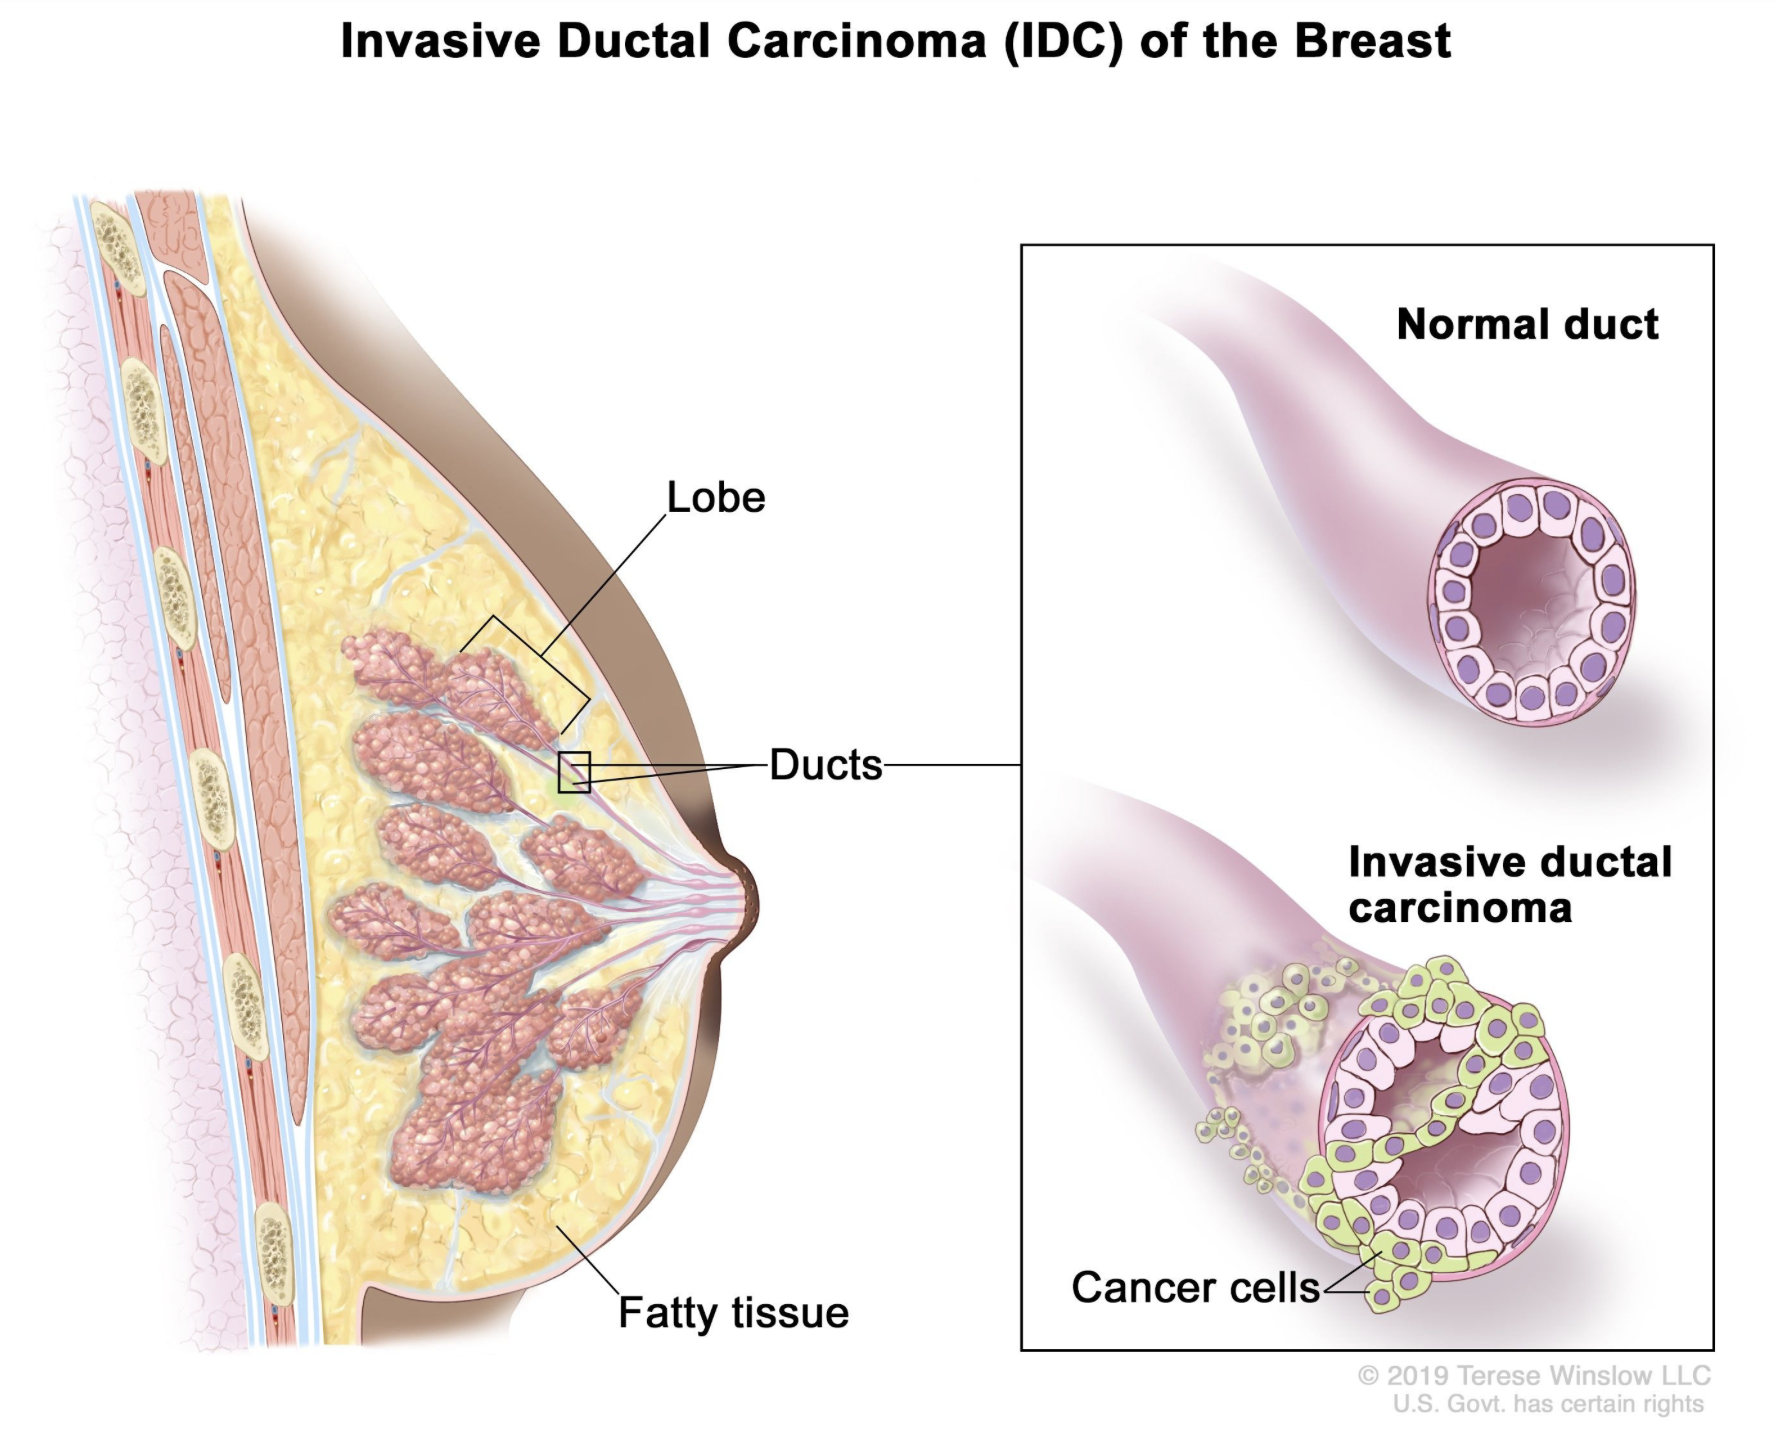
\includegraphics[width=1\linewidth,trim={0 1.5cm 0 4.25cm},clip]{./imgs/idc}
  \begin{center}
          {\small \textbf{Figure 1.} A visual overview of IDC morphology retrieved from cancer.gov.}
   \end{center}
            
       Since the American Cancer Society estimates that 80\% of new breast cancer diagnoses in 2025 will be Invasive Ductal Carcinoma (IDC), we decided to work with IDC.
      For patients with IDC, the AC treatment (comprises doxorubicin and cyclophosphamide) is the most common chemo treatment administered.
      We decided to look only at Natural Killer (NK) and  CD8$^+$ T cells since these two are the main immune cells attacking the majority of breast cancers [ABZ21].
      Moreover, from what we learned in our last cancer modeling project, we decided to also look at the population of normal cells, which for IDC are the normal epithelial cells of the milk duct where IDC begins.\\
      
The AC treatment is typically given in doses spread across, at most, 126 days.
The dosage of AC administered to a patient primarily depends on several factors like height, weight, cancer cell count amongst others.
Furthermore, the purpose of AC is treat early-stage localized breast cancer by killing cancer from inside the cells, damaging the DNA of cancer cells, and stopping their reproduction [Breast Cancer.org].
Thus, we need to also look some point after 126 days to see if the total IDC cell count is eradicated or low enough so that the immune system can kill any remaining cells.

            \columnbreak
            
\vspace{1mm}

\begin{center}
        \LARGE{\textbf{Modeling Assumptions \& Equations}}
\end{center}
\large
\vspace{-2mm}

           
Let $T(t)$ be the IDC burden at time $t$,  with $t$ measured in days, $N(t)$ be the cell count of normal epithelial cells, $CD(t)$ be the CD8$^+$ cell count, and $NK(t)$ be the count of NK cells.
Denote the state vector as $\x(t) = \begin{bmatrix}T & N & CD & NK\end{bmatrix}^{\trp}$.
We decided to model competition between the $N$ and $T$ as well as the growth for both following Gompertzian growth.
We also decided to add Michaelis-Menten kinetics to factor in tumor cell lysis and immune cell recruitment in both NK and CD.
Since IDC starts off localized, we decided to consider the natural death of both immune cells and some constant inflow rate of these into the ductal region.
Lastly, we also added in death rates that either come naturally or by interaction for all cells
Thus, components of our state evolve according to
            \begin{align*}
           	 \frac{\diff T(t)}{\diff t} = g_T T \ln &\Bigl( \frac{T_{\max}}{T} \Bigr)- a_1NT - a_2NKT - a_3CDT -\Bigl( E_c D_c  +\frac{4}{5}E_d D_d\Bigr) T, \\
            	\frac{\diff N(t)}{\diff t} &= g_N N \ln\Bigl(\frac{N_{\max}}{N} \Bigr) - k_N N - a_0NT, \\
		\frac{\diff CD(t)}{\diff t} &= r_{CD} - k_{CD} CD - \frac{\rho_0 CDT ^ i}{\alpha_0 + T^i} - a_4CDT - b_{CD}D_cCD, \\
	         \frac{\diff NK(t)}{\diff t} &=r_{NK} - k_{NK} NK - \frac{\rho _1NKT^i}{\alpha_1 + T^i} - a_5 NK T.
            \end{align*}

Denote the control $\mathbf{u}(t)=\begin{bmatrix} D_c(t) & D_d(t) \end{bmatrix}^{\trp}$ where $D_d$ is the drug concentration of doxorubicin and $D_c$ the drug concentration of cyclophosphamide, and both are measured in  $\frac{\text{mg}}{\text{m}^2} $.
To simplify the chemotherapy, we decided to use the average height and average weight of a  65 year old woman.
This helps us find constraints that our optimal control must satisfy, which are
\[
\begin{bmatrix} 0\\  0  \end{bmatrix} \leq \mathbf{u} \leq \begin{bmatrix} 1,700\\  127.5  \end{bmatrix} \\
\]

        \begin{center}
        \vspace{2cm}
        \LARGE{\textbf{The Cost Functional}}
        \end{center}
         	\large
         
We consider the problem of finding an optimal AC treatment for a total of 156 days.
The first 126 days corresponde to the normal AC treatment schedule and the last 30 days will be used to monitor how much cancer is remaining. 
The hope is that either the cancer will be eradicated after 126 days or that remainder can be handled by the interactions of the immune cells within 30 days.
Our cost functional (the OTC performance criterion) takes the form of 
\begin{align*}
	J[\mathbf{u}] = \int_0^{126}\mathbf{u}(t)^{\trp} Q \mathbf{u}(t)+ T^2(t) \diff t + \xi_{126} T^2(126)
\end{align*}
where $Q = \begin{bmatrix} \xi_c & 0 \\ 0 & \xi_d \end{bmatrix}$ denotes the positive weights for each of the elements of $\mathbf{u}$ and similarly for $ \xi_{126}$.\\

The Lagrangian $L(t, \x(t),\mathbf{u}(t))=\mathbf{u}^{\trp} Q \mathbf{u}+ T^2$ helps us take into consideration the fact we do not want to overdose a person as we administer the chemo as well as incorporating the number of IDC cells present through out the treatment.
The endpoint cost of $\phi(\x(126)) = \xi_{126} T^2(126)$ will help us ensure we penalize the final population of $T$ once the treatment is done. 

\vspace{-6mm}
    \FancySubtitle[0cm][2cm]{The Approach}
            \large 

Before we can begin finding an optimal control, we needed to find a way to incorporate the hard constraints that $\mathbf{u}$ must follow. 
Our initial approach was to incorporate those into our cost functional; that is, we decided to modify them as soft constraints.
We added $\frac{\alpha}{1 + (D - \text{bound})^{\lambda}}$ into our cost functional, where $\alpha$ helps is give a cost to each bound, not all necessarily the same, and $\lambda$ helps us control how much the difference between the dosage $D$ and the bound (lower or upper) matters.\\
            

Having incorporated our constraints into our functional, we first sought to apply Pontryagin's Maximum Principle which states that an optimal control $\tilde{\mathbf{u}}$ satisfies $\frac{DH}{D\mathbf{u}} = \mathbf{0}$, where $H(t, \x(t), \mathbf{u}(t),\mathbf{p}(t)) = \mathbf{p}\cdot \x^\prime - L$.



    \FancySubtitle[4mm][1cm]{Early Results \& Analysis}
    
        \begin{center}
          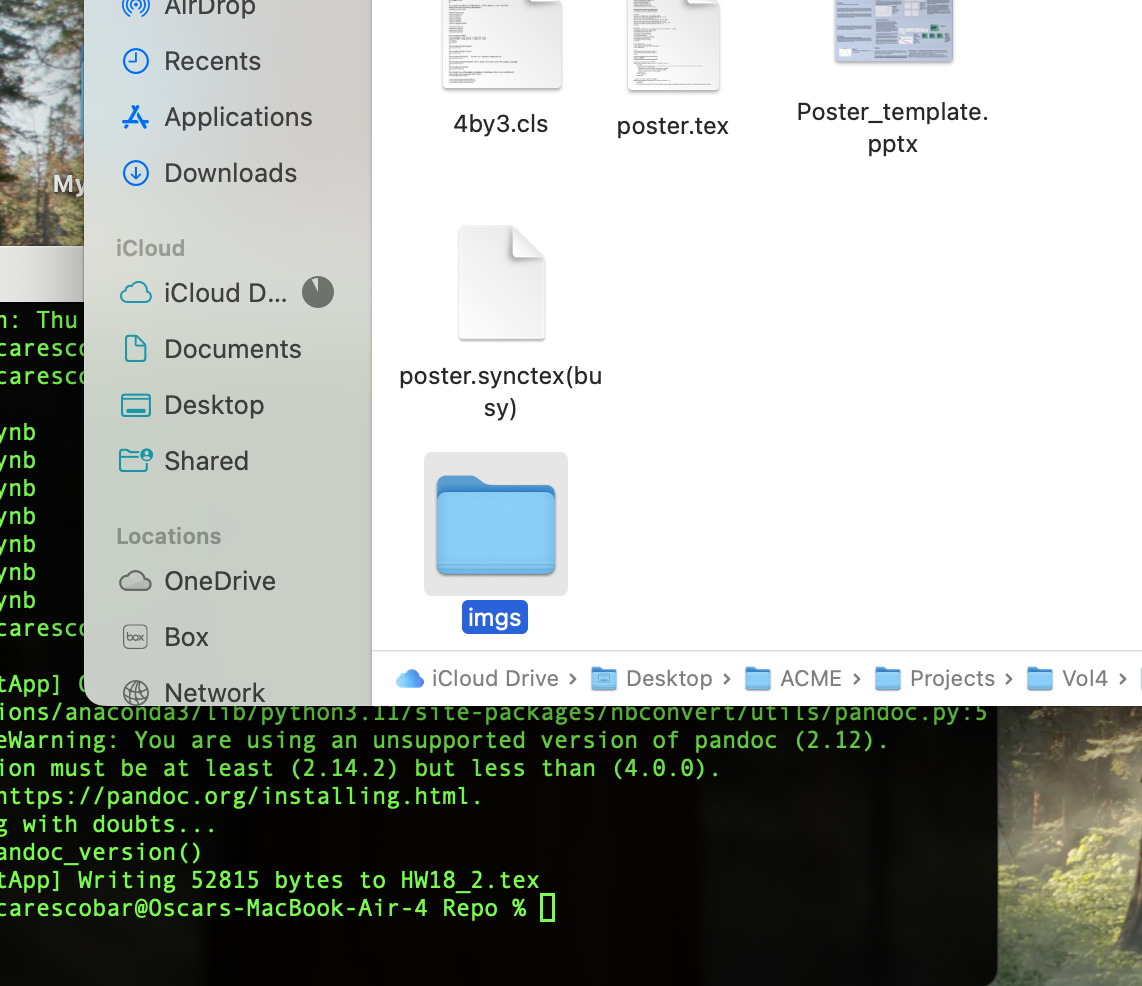
\includegraphics[width=1\linewidth,trim={0 8cm 0 10cm},clip]{./imgs/img.png}
        \end{center}
        


          \columnbreak  
 As the sun dipped below the horizon, casting hues of orange and pink across the sky, the quaint village came to life with the soft chatter of its inhabitants. Children chased each other through narrow cobblestone streets, their laughter echoing against the ancient stone walls. The scent of freshly baked bread wafted from the local bakery, enticing passersby with its warm embrace. In the distance, the sound of church bells rang out, signaling the end of another peaceful day in this idyllic countryside retreat.

   \FancySubtitle[4mm][1cm]{Conclusions and next steps}
  As the sun dipped below the horizon, casting hues of orange and pink across the sky, the quaint village came to life with the soft chatter of its inhabitants. Children chased each other through narrow cobblestone streets, their laughter echoing against the ancient stone walls. The scent of freshly baked bread wafted from the local bakery, enticing passersby with its warm embrace. In the distance, the sound of church bells rang out, signaling the end of another peaceful day in this idyllic countryside retreat.
 As the sun dipped below the horizon, casting hues of orange and pink across the sky, the quaint village came to life with the soft chatter of its inhabitants. Children chased each other through narrow cobblestone streets, their laughter echoing against the ancient stone walls. The scent of freshly baked bread wafted from the local bakery, enticing passersby with its warm embrace. In the distance, the sound of church bells rang out, signaling the end of another peaceful day in this idyllic countryside retreat.

    \bibliographystyle{amsalpha}
    \bibliography{poster_references}
\end{multicols*}
\end{minipage}

\nocite{unsplash}
%Using nocite allows a reference to appear in the reference list without a citation appearing in the poster.
\footnotesize

\end{document}